% Pipeline figure for §3. Shows: cipher BLIF -> three representations ->
% fault campaign -> three measured metrics, plus a side branch for the FPGA
% evaluation. Self-contained tikz block; \input it from §3 inside a figure.

\begin{figure*}[tbp]
  \centering
  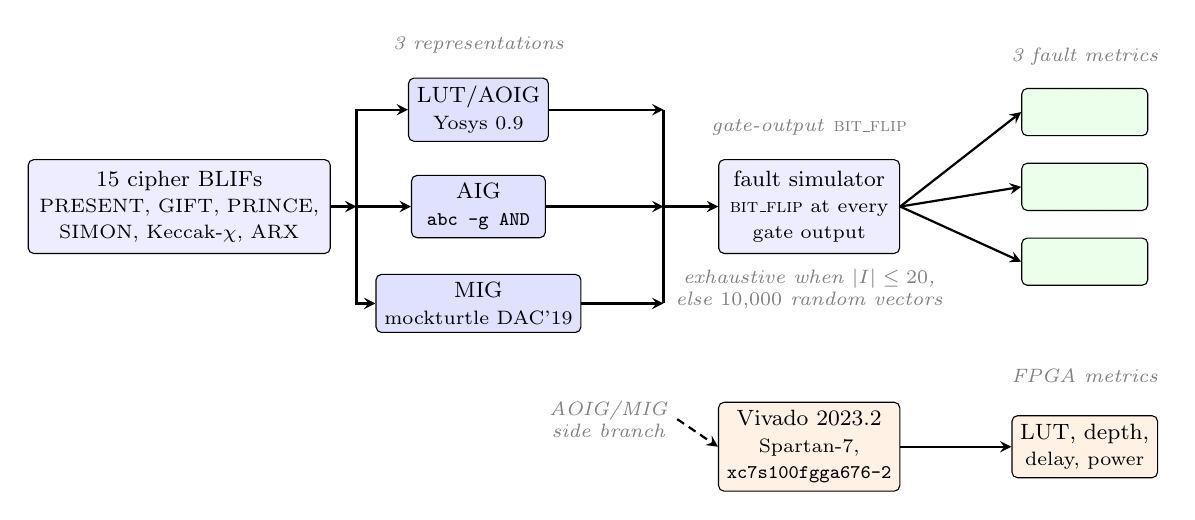
\begin{tikzpicture}[
    >=stealth,
    every node/.style={font=\footnotesize},
    block/.style={draw, rounded corners=2pt, minimum width=2.0cm,
                  minimum height=0.75cm, align=center, fill=blue!7,
                  inner sep=4pt},
    flow/.style={draw, rounded corners=2pt, minimum width=1.7cm,
                 minimum height=0.6cm, align=center, fill=blue!12,
                 inner sep=3pt},
    metric/.style={draw, rounded corners=2pt, minimum width=1.6cm,
                   minimum height=0.6cm, align=center, fill=green!8,
                   inner sep=3pt},
    fpga/.style={draw, rounded corners=2pt, minimum width=1.6cm,
                 minimum height=0.6cm, align=center, fill=orange!10,
                 inner sep=3pt},
    arrow/.style={->, thick},
    bus/.style={thick},
    note/.style={font=\scriptsize\itshape, gray},
  ]

    % ----- INPUT -----
    \node[block] (cipher) at (0, 0) {15 cipher BLIFs\\
        \scriptsize PRESENT, GIFT, PRINCE,\\
        \scriptsize SIMON, Keccak-$\chi$, ARX};

    % ----- THREE REPRESENTATIONS -----
    \node[flow] (aoig) at (3.8,  1.23) {LUT/AOIG\\\scriptsize Yosys 0.9};
    \node[flow] (aig)  at (3.8,  0.00) {AIG\\\scriptsize \texttt{abc -g AND}};
    \node[flow] (mig)  at (3.8, -1.23) {MIG\\\scriptsize mockturtle DAC'19};

    \coordinate (split) at (2.25, 0);
    \draw[arrow] (cipher.east) -- (split);
    \draw[arrow] (split) |- (aoig.west);
    \draw[arrow] (split) |- (aig.west);
    \draw[arrow] (split) |- (mig.west);

    % ----- COMMON FAULT CAMPAIGN -----
    \node[block] (sim) at (8.0, 0) {fault simulator\\
        \scriptsize \textsc{bit\_flip} at every\\
        \scriptsize gate output};

    \coordinate (faultbus) at (6.15, 0);
    \draw[bus] (faultbus |- aoig.east) -- (faultbus |- mig.east);
    \draw[arrow] (aoig.east) -- (faultbus |- aoig.east);
    \draw[arrow] (aig.east) -- (faultbus |- aig.east);
    \draw[arrow] (mig.east) -- (faultbus |- mig.east);
    \draw[arrow] (faultbus) -- (sim.west);

    % ----- METRICS -----
    \node[metric] (fc)   at (11.5,  1.2) {\FCpct};
    \node[metric] (avgdp) at (11.5, 0.25) {\AvgDP};
    \node[metric] (avgbw) at (11.5, -0.7) {\AvgBW};

    \draw[arrow] (sim.east) -- (fc.west);
    \draw[arrow] (sim.east) -- (avgdp.west);
    \draw[arrow] (sim.east) -- (avgbw.west);

    % ----- FPGA SIDE-CAMPAIGN -----
    \node[fpga] (vivado) at (8.0, -3.05) {Vivado 2023.2\\
        \scriptsize Spartan-7,\\
        \scriptsize \texttt{xc7s100fgga676-2}};
    \node[fpga] (fpga_metrics) at (11.5, -3.05) {LUT, depth,\\
        \scriptsize delay, power};

    \node[note, align=center] (fpga_src) at (5.45, -2.7)
      {AOIG/MIG\\side branch};
    \draw[arrow, densely dashed] (fpga_src.east) -- (vivado.west);
    \draw[arrow] (vivado.east) -- (fpga_metrics.west);

    % ----- LABELS -----
    \node[note] at (3.8, 2.05) {3 representations};
    \node[note] at (8.0, 1.0) {gate-output \textsc{bit\_flip}};
    \node[note] at (11.5, 1.9) {3 fault metrics};
    \node[note] at (11.5, -2.15) {FPGA metrics};

    % ----- TEST-VECTOR ANNOTATION -----
    \node[note, align=center] at (8.0, -1.05)
      {exhaustive when $|I| \le 20$,\\else $10{,}000$ random vectors};

  \end{tikzpicture}
  \caption{Measurement pipeline. Each of 15 cipher BLIFs is synthesized
  through three logical representations. The fault simulator injects a single \bitflip{}
  at every gate output of every netlist on every test vector
  (exhaustive when feasible; $10{,}000$ uniform random vectors
  otherwise), producing all-site and target-layer metrics
  (\FCpct{}, \AvgDP{}, \AvgBW). The FPGA side-branch reports LUT,
  depth, delay, and power for context on AOIG/MIG; the fault
  analysis is independent of FPGA tooling.}
  \label{fig:pipeline}
\end{figure*}
